\cite{exos_oraux} p. 259 \& \cite{oraux_x_ens_3} p. 322

\begin{lemme}
    Soit $f : \Rp \to \R$ telle que, pour tout $a > 0$, la suite $\big(f(na) \big)_{n \geqslant 0}$ tend vers 0.
    \item Montrer que si la fonction $f$ est uniformément continue, on a $\lim\limits_{x \to + \infty} f(x) = 0$.
\end{lemme}

correction principalement de \cite{oraux_x_ens_3} mais avec des précisions venant de \cite{exos_oraux}.

\begin{preuve}
    L'hypothèse signifie que $f$ tend vers $0$ selon toute suite arithmétique de la forme $(na)_{n \geqslant 0}$. Lorsque la fonction est uniformément continue, on peut contrôler son comportement entre deux termes consécutifs de la suite. Plus précisément, soit $\varepsilon > 0$. La continuité uniforme de $f$ permet de choisir $\eta_\varepsilon > 0$ tel que pour tout $(x, y) \in (\Rp)^2$, 
    $$|x-y| \leqslant \eta_\varepsilon \Rightarrow |f(x) - f(y)| \leqslant \varepsilon.$$
    Puisque $\eta_\varepsilon > 0$, la suite $\big(f(n\eta_\varepsilon)\big)_{n \geqslant 0}$ tend vers $0$ par hypothèse. Fixons $N$ tel que $|f(n \eta_\varepsilon)| \leqslant \varepsilon$ pour $n \geqslant N$. \\
    Soient $x \geqslant N \eta_\varepsilon$ et $n \defeq \min\{ k \in \N | x \leqslant k \eta_\varepsilon \}$ qui est bien défini. Alors $|x-n\eta_\varepsilon| \leqslant \eta_\varepsilon$. On a alors $|f(x) - f(n \eta_\varepsilon)| \leqslant \varepsilon$ de sorte que par l'inégalité triangulaire, 
    \begin{align*}
        |f(x)| &\leqslant |f(x) - f(n \eta_\varepsilon)| + |f(n \eta_\varepsilon)| \\
        &\leqslant 2 \varepsilon.
    \end{align*}
    Ceci étant valable pour tout $x \geqslant N \eta_\varepsilon$, on a bien prouvé que $f$ tend vers $0$ en $+ \infty$.
\end{preuve}  

\begin{marginfigure}[-3cm]
    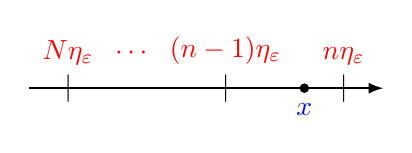
\begin{tikzpicture}[scale=5]
    \draw[-latex] [thick](-0.1,0) -- (0.8,0);
    
    \draw (0,0) node [above=5pt, red,fill=white]{$N \eta_\varepsilon$};
    \draw (0,0) node {$|$};
    
    \draw (0.16,0) node [above=7pt, red,fill=white]{$\cdots$};

    \draw (0.4,0) node [above=5pt, red,fill=white]{$(n-1) \eta_\varepsilon$};
    \draw (0.4,0) node {$|$};
    
    \draw [fill] (0.6,0) circle [radius=0.3pt];
    \draw (0.6,0) node [below=2pt, blue,fill=white]{$x$};

    \draw (0.7,0) node [above=5pt, red,fill=white]{$n \eta_\varepsilon$};
    \draw (0.7,0) node {$|$};
\end{tikzpicture}
\end{marginfigure}
